\chapter{Polimorfismo, Herencia y Delegación}

En esta unidad veremos algunos temas que son centrales a la programación
orientada a objetos: polimorfismo, herencia y delegación.

\section{Polimorfismo}

El concepto de {\it polimorfismo} (del griego {\it muchas formas}) implica
que si en una porción de código se invoca un determinado método de un
objeto, podrán obtenerse distintos resultados según la clase del objeto.
Esto se debe a que distintos objetos pueden tener un método con un mismo
nombre, pero que realice distintas operaciones.

En las unidades anteriores, varias veces utilizamos las posibilidades
provistas por el polimorfismo, sin haberle puesto este nombre. Algunos
ejemplos:

\begin{itemize}
\item Es posible recorrer cualquier tipo de secuencia
(ya sea una lista, una tupla, un diccionario, un archivo o cualquier otro tipo
de secuencia) utilizando la misma estructura de código:
|for elemento in secuencia|.

\item Se puede obtener la cantidad de
elementos de cualquier secuencia utilizando la misma función: |len(secuencia)|.

\item Varias funciones y operaciones pueden trabajar con los
distintos tipos numéricos sin hacer distinción sobre de qué tipo de número
se trataba (entero, real, largo o complejo); por ejemplo |abs(numero)|.

\item La función |str| permite convertir cualquier objeto a una representación
en cadena de texto, sin importar el tipo del objeto.
\end{itemize}

Todos los casos mencionados son ejemplos de polimorfismo: la misma operación
produce resultados diferentes (o el mismo resultado, pero que se calcula de
manera diferente) según el tipo de objeto al que se aplica la operación.

\subsection{Interfaz}

Llamamos {\bf interfaz} a un conjunto de funciones, métodos o atributos con
nombres específicos.  Una interfaz es un {\it contrato} entre el
programador que realiza una clase y el que la utiliza, y puede consistir en
uno solo o varios métodos o atributos.

Por ejemplo, para que un objeto se pueda sumar con otro utilizando el
operador |+|, debe cumplir con la interfaz {\it sumable}, que en Python
implica incluir el método |__add__| visto en la unidad anterior.

Una manera de implementar polimorfismo es utilizar distintos tipos de
datos a través de una interfaz común. Por ejemplo, cuando sumamos dos
objetos |a| y |b| con la expresión:

\begin{codigo-python-sn}
a + b
\end{codigo-python-sn}

\noindent no es necesario que sepamos de qué tipo son los objetos; si
alguno de los dos cumple con la interfaz {\it sumable}, podemos decir
que la operación será exitosa y producirá algún resultado.

\subsection{Redefinición de métodos}

Llamamos {\bf redefinición} a la acción de definir un método con el mismo
nombre en distintas clases, de forma tal que provea una interfaz.

Un bloque de código será {\it polimórfico} cuando dentro de ese código se
realicen llamadas a métodos que puedan estar redefinidos en distintas
clases.

Tomemos por ejemplo el caso ya mencionado en el que se recorre una
secuencia (lista, tupla, archivo, etc) mediante una misma estructura de
código.  Esto es posible gracias a la redefinición del método especial
\lstinline!__iter__!, que devuelve un {\it iterador}.  Un bloque que
utiliza una secuencia en forma genérica es, entonces, un bloque
polimórfico.

\begin{sabias_que}
En Python, al no ser necesario especificar explícitamente el tipo de los
parámetros que recibe una función, todas las funciones son naturalmente
polimórficas.

En otros lenguajes puede darse que sólo algunas funciones específicas sean
polimórficas (como en C++, por ejemplo), o que sea extremadamente difícil
obtener un comportamiento polimórfico (como es el caso de C).
\end{sabias_que}

En la vida real, cuando analizamos las funciones de respiración,
reproducción o alimentación de los seres vivos vemos que siempre se repite
el mismo patrón: si bien la acción en todos los casos es la misma, puede
suceder que haya diferencias en la {\it implementación} en cada tipo, ya
que la respiración de una mojarrita que la de un malvón no funcionan de la
misma manera, o tampoco así la reproducción de una ameba y la de un elefante.

Análogamente, al implementar nuestras clases podemos proveer
distintas implementaciones para un método con el mismo nombre, para que
puedan comportarse polimórficamente, como ser las redefiniciones de los
métodos \lstinline!__str__! o \lstinline!__lt__!.

En particular en Python, la {\it sobrecarga de operadores} (mencionada
en la sección \ref{sobrecarga}),  es un proceso que se realiza mediante la
redefinición de
algunos métodos especiales.  En otros lenguajes se utilizan técnicas distintas
para obtener el mismo resultado.

\begin{sabias_que}
El término {\it sobrecarga} viene de un posible uso de polimorfismo que
está presente en algunos lenguajes orientados a objetos: la posibilidad de
tener, dentro de una misma clase, dos métodos que se llamen igual pero
reciban parámetros de distintos tipos.  Es decir, que el método al que hay
que llamar se decide por el tipo del parámetro, no por el tipo del objeto
que lo contiene.

En Python no tenemos sobrecarga de métodos, ya que al no definir los tipos
de los parámetros en el encabezado, no sería posible distinguir a qué
método hay que llamar.  Sin embargo, se puede decir que sí tenemos
sobrecarga de operadores, ya que al encontrar un operador, Python llamará a
distintos métodos según el tipo de las variables que se quiera sumar,
restar, multiplicar, etc.
\end{sabias_que}

\subsection*{Ejemplos de polimorfismo}

En la unidad anterior se vio la clase \lstinline!Punto! que representa a un
punto en el plano.  Es posible definir también una clase
\lstinline!Punto3D!, que represente un punto en el espacio.  Esta nueva
clase contendrá los mismos métodos que se vieron para \lstinline!Punto!,
pero para tres coordenadas.

Si a ambas clases le agregamos un método para dividir por un escalar
(\lstinline!__div__(self, escalar)!), podríamos tener la siguiente función
polimórfica:

\begin{codigo-python-sn}
def obtener_versor(punto):
    return punto / punto.norma()
\end{codigo-python-sn}

Esta función devolverá un versor de dos dimensiones o de tres dimensiones,
según a qué clase pertenezca la variable \lstinline!punto!.

\begin{atencion}
Que una función sea polimórfica no significa que pueda operar sobre parámetros
de {\it cualquier} tipo de dato, sino que suele imponer restricciones.  En el
ejemplo anterior, las restricciones son que el objeto |punto| tenga el método
|norma| y la posibilidad de dividirlo por un escalar.
\end{atencion}

Veamos otro ejemplo: una función que cuenta la frecuencia de aparación de
elementos dentro de una secuencia cualquiera.

\begin{codigo-python-sn}
def frecuencias(secuencia):
    """Calcula las frecuencias de aparición de los elementos de
       la secuencia recibida.
       Devuelve un diccionario con elementos: {valor: frecuencia}
    """
    frec = {}
    for elemento in secuencia:
        frec[elemento] = frec.get(elemento, 0) + 1
    return frec
\end{codigo-python-sn}

Vemos que el parámetro \lstinline!secuencia! puede ser de cualquier tipo
que se encuentre dentro de la ``familia'' de las secuencias. En cambio, si
llamamos a la función con un entero se levanta una excepción.

\begin{codigo-python-sn}
>>> frecuencias(["peras", "manzanas", "peras", "manzanas", "uvas"])
{'uvas': 1, 'peras': 2, 'manzanas': 2}
>>> frecuencias((1, 3, 4, 2, 3, 1))
{1: 2, 2: 1, 3: 2, 4: 1}
>>> frecuencias("Una frase")
{'a': 2, ' ': 1, 'e': 1, 'f': 1, 'n': 1, 's': 1, 'r': 1, 'U': 1}
>>> frecuencias(range(3, 10, 2))
{9: 1, 3: 1, 5: 1, 7: 1}
>>> frecuencias(4)
Traceback (most recent call last):
  File "<pyshell#0>", line 1, in <module>
    frecuencias(4)
  File "frecuencias.py", line 12, in frecuencias
    for elemento in secuencia:
TypeError: 'int' object is not iterable
\end{codigo-python-sn}

\section{Herencia}

Otro mecanismo de la programación orientada a objetos que permite implementar
comportamientos polimórficos es la {\it herencia}, que permite crear clases
nuevas a partir de clases preexistentes.  Mediante la herencia, una clase puede
{\it extender} a otra y de esta manera {\it heredar} sus atributos y
comportamientos, pudiendo modificarlos para implementar un comportamiento
diferente.

La clase vieja se llama {\it clase base} y la que se construye a partir de
ella es una {\it clase derivada}.

Por ejemplo, a partir de una clase \lstinline!Persona! con los atributos
\lstinline!identificacion!, \lstinline!nombre! y \lstinline!apellido!,
podemos construir la clase \lstinline!AlumnoFIUBA! que extiende a
\lstinline!Persona! y agrega como atributo el \lstinline!padron!.

Definamos primero la clase base, |Persona|:

\begin{codigo-python-sn}
class Persona:
    def __init__(self, identificacion, nombre, apellido):
        self.identificacion = identificacion
        self.nombre = nombre
        self.apellido = apellido

    def __str__(self):
        return "{}: {}, {}".format(
            self.identificacion, self.apellido, self.nombre
        )
\end{codigo-python-sn}

A continuación definimos |AlumnoFIUBA|, indicando entre paréntesis que la clase
base es |Persona|:

\begin{codigo-python-sn}
class AlumnoFIUBA(Persona):
    def __init__(self, identificacion, nombre, apellido, padron):
        super().__init__(identificacion, nombre, apellido)
        self.padron = padron
\end{codigo-python-sn}

En la primera línea del constructor invocamos al constructor de |Persona|,
pasándole los parámetros necesarios (si no hiciéramos esto, las instancias de
|AlumnoFIUBA| no tendrían los atributos |identificacion|, |nombre| o
|apellido|). En la segunda línea asignamos el atributo |padron|.

Probamos la nueva clase:

\begin{codigo-python-sn}
>>> a = AlumnoFIUBA("DNI 35123456", "Damien", "Thorn", "98765")
>>> str(a)
'DNI 35123456: Thorn, Damien'
\end{codigo-python-sn}

Vemos que se heredó el método \lstinline+__str__+ de la clase base. Si
queremos, podemos redefinirlo:

\begin{codigo-python-sn}
    def __str__(self):
        return "Padrón {}: {}, {}".format(
            self.padron, self.apellido, self.nombre
        )
\end{codigo-python-sn}

\begin{codigo-python-sn}
>>> a = AlumnoFIUBA("DNI 35123456", "Damien", "Thorn", "98765")
>>> str(a)
'Padrón 98765: Thorn, Damien'
\end{codigo-python-sn}

De una clase base se pueden construir muchas clases derivadas: así como
hemos derivado alumnos, podríamos derivar docentes, empleados, clientes,
proveedores, o lo que fuera necesario según la aplicación que estemos
desarrollando. Incluso podríamos aplicar más de un nivel de herencia: |B|
extiende |A|, |C| extiende |B|, \ldots

\begin{sabias_que}
En el diseño de jerarquias de herencia no siempre es del todo fácil decidir
cuándo una clase debe extender a otra.
Una regla práctica para decidir si una clase |S| puede ser
definida como heredera de otra |T| es que debe cumplirse que ``S es un T''.
Por ejemplo, {\it Perro} es un {\it Animal}, pero {\it Vehículo} no es un {\it
Motor}.

Esta regla se desprende del principio de sustitución de Liskov (formulado por
Barbara Liskov y Jeannette Wing).

Barbara Liskov es una mujer importante en la historia de la informática, no
sólo por este principio, sino que fue la primera mujer en recibir un doctorado
en las ciencias de la computación, creadora de varios lenguajes y actualmente
es profesora e investigadora del MIT.
\end{sabias_que}

En el caso de Python, también es posible construir una clase derivada a partir
de varias clases base. Por ejemplo, un ayudante de segunda en la UBA es un
alumno que también trabaja de docente.  Esta posbilidad se llama {\it herencia
múltiple}.

\subsection*{Ejemplo de herencia}

Un ejemplo clásico de herencia es el de las figuras geométricas: todas las
figuras tienen un nombre y un color, pero cada figura diferente puede tener
atributos diferentes como radio, base, altura, etc., y una fórmula diferente
para calcular el área.

\begin{itemize}
\item La clase base:

\begin{codigo-python-sn}
class Figura(object):
    def __init__(self, nombre, color):
        self.nombre = nombre
        self.color = color

    def area(self):
        raise NotImplementedError("Este método debe ser redefinido.")

    def __str__(self):
        return "<{} - color: {} - área: {:.2f}>".format(
            self.nombre, self.color, self.area()
        )
\end{codigo-python-sn}

\item Los círculos:

\begin{codigo-python-sn}
from math import pi

class Circulo(Figura):
    def __init__(self, radio, color):
        super().init("Círculo", color)
        self.radio = radio

    def area(self):
        return pi * self.radio * self.radio
\end{codigo-python-sn}

\item Y los triángulos:

\begin{codigo-python-sn}
class Triangulo(Figura):
    def __init__(self, base, altura, color):
        super().init("Triángulo", color)
        self.base = base
        self.altura = altura

    def area(self):
        return self.base * self.altura / 2
\end{codigo-python-sn}

\end{itemize}

Y ahora las pruebas:

\begin{codigo-python-sn}
>>> c = Circulo(4, "verde")
>>> str(c)
'<Círculo - color: verde - área: 50.27>'
>>> t = Triangulo(3, 5, "azul")
>>> str(c)
'<Triángulo - color: azul - área: 7.5>'
\end{codigo-python-sn}

\section{Delegación}

Llamamos delegación a la situación en la que una clase contiene (como
atributos) una o más instancias de otra clase, a las que {\it delegará}
parte de sus funcionalidades. Esta relación entre clases suele ser la más
indicada cuando es necesaria una asociación entre las clases pero el
principio de Liskov no se cumple. También puede verse como la relación
entre clases ``S contiene a T''. Por ejemplo, Vehículo {\bf contiene} un
Motor, pero Alumno no contiene a Persona, sino que {\bf es} una Persona.

Por ejemplo, la clase \lstinline!Hotel! vista en la unidad anterior, podría
contener una instancia de \lstinline!Disponibilidad!, que almacene la
disponibilidad de las habitaciones del hotel para distintas fechas.  La
clase \lstinline!Hotel! debería tener, entonces, los métodos
\lstinline!consultar_disponibilidad!, \lstinline!reservar! y
\lstinline!cancelar!, que todos delegarían en la clase
\lstinline!Disponibilidad! su funcionamiento principal.

% TODO: completar el ejemplo.

%\ejercicioc{Programar una clase \verb+DisponibilidadHotel+ contenida en \verb+Hotel+
%que tenga un calendario de disponibilidades de un hotel y donde se puedan hacer
%reservas para una fecha dada.}

%\ejercicioc{Se necesita una clase que permita ver la disponibilidad hotelera
%de una ciudad,
%y que cuente con un método {\tt aconsejar} que, para una
%fecha dada, aconseje cuáles son los hoteles disponibles ordenados de mayor
%a menor por la relación calidad--precio. Debe permitir reservar una habitación
%en el hotel elegido.}

\subsection*{Delegación y Referencias}

Queremos construir una clase \lstinline!Rectangulo!, que se describe
mediante los siguientes atributos:

\begin{itemize}
\item {\bf Longitud de su base}: un número.

\item {\bf Longitud de su altura}: un número.

\item {\bf El punto del plano de su esquina inferior izquierda}: un punto del plano.

\end{itemize}

Incluiremos métodos para inicializar y mostrar, para calcular el área y
para trasladar el rectángulo en el plano.

\begin{codigo}{Rectangulo.py}{Clase para modelar un Rectángulo}
\label{Rectangulo}
\lstinputlisting{src/15_herencia_polimorf/Rectangulo.py}
\end{codigo}

La implementación básica puede verse en el Código \ref{Rectangulo}.  Se
puede ver que el rectángulo realiza internamente la operación para calcular
el área, pero para la operación |trasladar|, delega la suma de los puntos
al operador \lstinline!__add__! de la clase \lstinline!Punto!
(recordamos que cuando se hace \lstinline!self.origen + Punto(dx,dy)!,
Python llama al método \lstinline!__add__! de la clase \lstinline!Punto!,
que recibe los dos puntos y devuelve un nuevo punto con la suma de ambos).

Para construir y utilizar el rectángulo, lo haremos de la siguiente forma:

\begin{codigo-python-sn}
>>> from Punto import Punto
>>> from Rectangulo import Rectangulo
>>> r = Rectangulo(Punto(1, 2), 2, 3)
>>> str(r)
Origen: (1, 2), Base: 2, Altura: 3
>>> r.area()
6
\end{codigo-python-sn}

Lo que acabamos de crear es un objeto de acuerdo al siguiente diagrama que
se muestra en la Figura \ref{rectangulo_punto}.

\begin{figure}[htb]
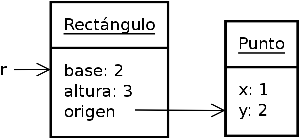
\includegraphics{graficos/15_Rectangulo_Punto}
\caption{Estado de las variables, al momento de crear el rectángulo}
\label{rectangulo_punto}
\end{figure}

El punto que describe la posición de la esquina inferior izquierda del
rectángulo es un objeto \lstinline!Punto!. El atributo \lstinline!origen!
contiene una {\it referencia} a dicho objeto.

Utilizando el método \lstinline!trasladar!, podemos modificar el valor del
punto contenido dentro del rectángulo.

\begin{codigo-python-sn}
>>> r.trasladar(2, 4)
>>> str(r)
Origen: (3, 6), Base: 2, Altura: 3
\end{codigo-python-sn}

También es posible directamente reemplazar el punto contenido, por un nuevo
punto.

\begin{codigo-python-sn}
>>> q = Punto(7, 2)
>>> r.origen = q
>>> str(r)
Origen: (7, 2), Base: 2, Altura: 3
\end{codigo-python-sn}

Con lo cual el diagrama pasa a ser el de la Figura
\ref{rectangulo_punto_b}.

\begin{figure}[htb]
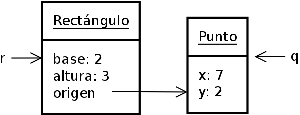
\includegraphics{graficos/15_Rectangulo_Punto_b}
\caption{Estado de las variables, luego de reemplazar el origen}
\label{rectangulo_punto_b}
\end{figure}

\begin{observacion}
El \lstinline!Punto(1, 2)! y \lstinline!Punto(3,6)! que habían sido creados
previamente, están ahora fuera de uso, por lo que quedan a disposición de un
mecanismo de {\it recolección de basura} que se encarga de recuperar
automáticamente las secciones de memoria que quedan fuera de uso durante la
ejecución de un programa.
\end{observacion}

\section{Resumen}

\begin{itemize}
\item Se llama {\bf polimorfismo} a la posibilidad de obtener distintos
comportamientos mediante la invocación a métodos de un mismo nombre, pero de
clases distintas.

\item Se llama {\bf herencia} a la relación entre clases en la cual una es una
clase base y otra es una clase derivada, que {\it hereda} los métodos y
atributos de la clase base.

\item Se llama {\bf delegación} a la relación entre clases en la cual una
instancia de una clase contiene como atributo una instancia de otra clase,
y dentro de sus métodos realiza invocaciones a los métodos de la clase
contenida.

\item Se denomina {\bf referencia} a las variables que permiten acceder a
un determinado objeto, ya sea un atributo dentro de un objeto, o una
variable en una porción de código cualquiera.
\end{itemize}


\newpage
\section{Ejercicios}

\extractionlabel{guia}
\begin{ejercicio}
{\bf Papel, Birome, Marcador}
\begin{partes}
    \item Escribir una clase {\it Papel} que contenga un texto, un método {\it
escribir}, que reciba una cadena para agregar al texto, y el método {\it
\_\_str\_\_} que imprima el contenido del texto.
    \item Escribir una clase {\it Birome} que contenga una cantidad de tinta, y
un método {\it escribir}, que reciba un texto y un papel sobre el cual
escribir. Cada letra escrita debe reducir la cantidad de tinta contenida.
Cuando la tinta se acabe, debe lanzar una excepción.
    \item Escribir una clase {\it Marcador} que herede de Birome, y agregue el
método {\it recargar}, que reciba la cantidad de tinta a agregar.
\end{partes}
\end{ejercicio}


\extractionlabel{guia}
\begin{ejercicio}
{\bf Juego de Rol}
\begin{partes}
    \item Escribir una clase {\it Personaje} que contenga los atributos {\it
vida}, {\it posicion} y {\it velocidad}, y los métodos {\it
recibir\_ataque}, que reduzca la vida según una cantidad recibida y lance
una excepción si la vida pasa a ser menor o igual que cero, y {\it
mover} que reciba una dirección y se mueva en esa dirección la cantidad
indicada por velocidad.
    \item Escribir una clase {\it Soldado} que herede de Personaje, y agregue
el atributo {\it ataque} y el método {\it atacar}, que reciba otro
personaje, al que le debe hacer el daño indicado por el atributo ataque.
    \item Escribir una clase {\it Campesino} que herede de Personaje, y agregue
el atributo {\it cosecha} y el método {\it cosechar}, que devuelva la
cantidad cosechada.
\end{partes}
\end{ejercicio}

